\begin{figure}[t]
\centering
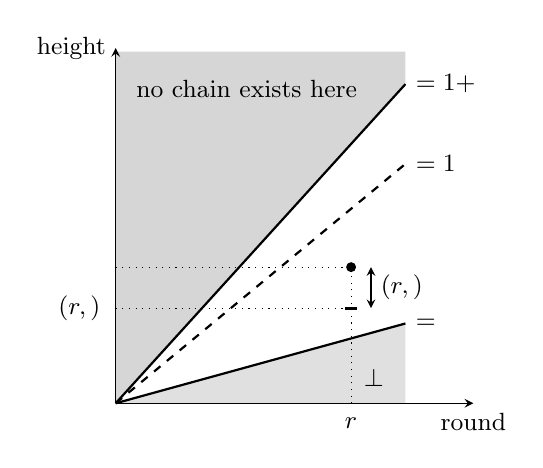
\begin{tikzpicture}[x=1.15cm,y=0.95cm,>=stealth,font=\small]
  % rho = 1/3: the three rays have slopes 4/3, 1 and 1/3.
  \def\xe{3.2}
  \def\yh{4.2667}   % top ray at \xe
  \def\ym{3.2}      % middle ray at \xe
  \def\yl{1.0667}   % bottom ray at \xe

  % regions
  \fill[black!12] (0,0) -- (\xe,\yl) -- (\xe,0) -- cycle;
  \fill[black!16] (0,0) -- (\xe,\yh) -- (\xe,4.7) -- (0,4.7) -- cycle;

  % axes
  \draw[->] (0,0) -- (3.95,0) node[below] {round};
  \draw[->] (0,0) -- (0,4.75) node[left] {height};

  % rays
  \draw[thick]        (0,0) -- (\xe,\yh) node[right] {$\rate=1+\advr$};
  \draw[thick,dashed] (0,0) -- (\xe,\ym) node[right] {$\rate=1$};
  \draw[thick]        (0,0) -- (\xe,\yl) node[right] {$\rate=\advr$};

  % the received chain at round r, of height alpha, and its confirmed prefix
  \def\xr{2.6}
  \def\ya{1.82}
  \def\yz{1.2711}
  \draw[dotted] (\xr,0) -- (\xr,\ya);
  \draw[dotted] (0,\ya) -- (\xr,\ya);
  \draw[dotted] (0,\yz) -- (\xr,\yz);
  \fill (\xr,\ya) circle (1.8pt);
  \draw[very thick] (\xr-0.07,\yz) -- (\xr+0.07,\yz);
  \draw[<->] (\xr+0.22,\yz) -- (\xr+0.22,\ya) node[midway,right] {$\prn(r,\hgt)$};

  \node[anchor=east] at (-0.06,\ya) {$\hgt$};
  \node[anchor=east] at (-0.06,\yz) {$\pref(r,\hgt)$};
  \node[anchor=north] at (\xr,-0.06) {$r$};

  \node[anchor=north west] at (0.12,4.45) {no chain exists here};
  \node at (2.85,0.34) {$\bot$};
\end{tikzpicture}
\caption{The confirmed height, drawn for $\advr=\frac{1}{3}$. A chain $\ch$ received
at round $r$ is a point at height $\hgt$. No chain reaches above the ray
$\rate=1+\advr$, and a chain adopted by an honest validator reaches at least
the ray $\rate=1$. The confirmed height $\pref(r,\hgt)$ interpolates linearly
between the two outer rays, equal to $\hgt$ on the upper one and to zero on the
lower one. The client prunes the difference $\prn(r,\hgt)$, and it outputs $\bot$
when the point falls below the lower ray.}\label{fig.confirmed}
\end{figure}
